\setchapterpreamble[o]{%
  \dictum[Steve Jobs]{\textit{``Design is not  just what it looks like and
      feels like. Design is how it works.''}}}

\chapter{Design and Implementation}
\label{cha:design}

This chapter is about the design and implementation of the \emph{Xen-based
  Execution  Environment} (\gls{glo:XenBEE}).   The  execution environment
incorporates  a total  of three  main  components: the  \emph{xbe} on  the
user's side, the \emph{xbed} on  the server's side and the \emph{xbeinstd}
on  the  side of  a  single virtual  machine.   All  components have  been
implemented     using    the     \emph{Python}     programming    language
\cite{python-language}. In particular, version  $2.5$ of that language has
been used.

Some additional  modules and programs, that  are not part  of the standard
libraries shipped with Python, have been used, though. Among these are for
instance  the \texttt{twisted}  framework \cite{twisted-python}  which has
been  used  for  the  network  code,  a  library  called  \texttt{libvirt}
\cite{libvirt}  that  was used  to  connect  to  the Xen  virtual  machine
monitor, and a library that  provides Python bindings to the \texttt{curl}
library \cite{pycurl}.


\section{Overview}
\label{sec:design:overview}

The picture in Figure~\ref{fig:architecture-overview} shows an overview of
the three components which, when put together, make up the \emph{Xen-based
  Execution Environment} (\gls{glo:XenBEE}).

\begin{figure}[ht]
  \centering
  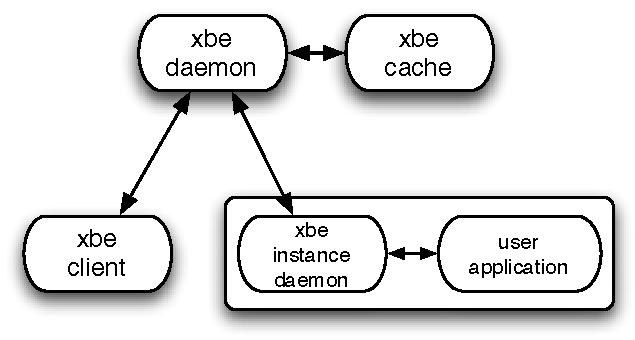
\includegraphics[scale=.7]{architecture-overview}
  \caption[Overview of the  \gls{glo:XenBEE} components]{The components of
    the Xen-based Execution Environment}
  \label{fig:architecture-overview}
\end{figure}

On the left hand side of the picture are the users using the \emph{xbe} to
communicate with the execution  environment. The \emph{xbe} refers in this
case  to the command  line tool  which I  have implemented  as a  proof of
concept  to interact  with the  \emph{xbed}.  The  interface that  an user
utilizes to execute his applications  with the \gls{glo:XenBEE} could be a
web-portal or some other tool with a graphical user interface, as well.

\medskip

On the right hand side are the components that are required to execute the
applications within  virtual machines.  The \emph{xbed} has  to be running
on a machine, that supports  the Xen hypervisor.  It maintains an internal
connection to  a local  cache, which can  be used  by any user  to deposit
arbitrary data on the  server side.  The \emph{xbed} uses \texttt{libvirt}
to connect to the Xen hypervisor and to manage active virtual machines.

Each virtual machine  must provide the \emph{xbeinstd}, that  means it has
to be started at some point during the initialization process of the guest
operating system. Any image that is submitted to the execution environment
must therefore  contain this  program. The \emph{xbeinstd}  is responsible
for two  major issues:  executing the actual  application and  keeping the
virtual machine instance alive.   Execution of an application involves for
instance  passing  arguments  to   the  executable,  setting  the  working
directory and redirecting the input and output streams. The \emph{xbed} is
going  to shut  stale virtual  machines down,  unless  the \emph{xbeinstd}
sends  regular keep-alive  messages  to the  \emph{xbed}.   If the  user's
application has finished, the \emph{xbeinstd} signals the \emph{xbed} that
the virtual machine is ready to be shut down.

\medskip

The  thicker connections  between \emph{xbe}  and \emph{xbed}  as  well as
between \emph{xbed}  and \emph{xbeinstd} are  logical connections realized
by using message-queues and one  or more \gls{glo:MQS} in between. Whereas
he  thinner links  are either  inner-process connections  (in case  of the
cache) or  connections between  parent and child  process (in case  of the
user-application).

\section[Xen-based Execution Daemon]{Xen-based Execution Daemon (xbed)}
\label{sec:xbed}

This  section describes  the  ``heart'' of  the  \gls{glo:XenBEE} ---  the
\emph{xbed}.  Well, the \emph{xbed}  is itself composed of several smaller
components that  are each responsible for  a single detail  of the daemon.
The    main    components    though    are   the    \texttt{Cache},    the
\texttt{TaskManager}  and the  \texttt{InstanceManager}. The  former  is a
rather simple implementation of a local data cache, that will be discussed
in a later section.

\begin{figure}[ht]
  \centering
  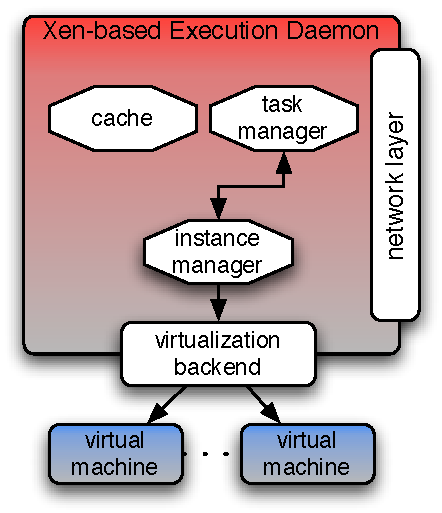
\includegraphics[scale=.55]{xbed-architecture}
  \caption[Components of the xbed]{The most important components of the xbed}
  \label{fig:xbed-architecture}
\end{figure}

\subsubsection{Network Layer}

On startup, the  daemon tries to connect to  the message-queue server that
has been  defined either in  its configuration file  or as a  command line
parameter. This process  is realized by the \emph{network  layer}. It uses
the  \texttt{twisted} framework to  establish a  \gls{glo:TCP} connection.
When the connection has been successfully established, a special transport
protocol --- the  STOMP protocol --- is attached  to the connection. STOMP
is  the \emph{Streaming  Text Oriented  Messaging Protocol}  and basically
defines a  very simple protocol to  send and receive text  messages over a
message-queue server.  On top of  this text message based protocol are XML
based  protocols  that  accomplish  the whole  communication  between  all
components.   There is currently  a basic  XML protocol  that encapsulates
single ``messages'', consisting just of header and body, and two protocols
that  connect up  the \emph{xbe}  and the  \emph{xbeinst}  accordingly.  A
special  protocol providing  security  related services  (\ie privacy  and
validity) can be added as an additional layer.

Anyway, the  details of the \gls{glo:STOMP}  and XML protocols  as well as
the network layer,  which is to some extent equal  among all components of
the        \gls{glo:XenBEE},       will       be        discussed       in
Section~\ref{sec:communication-protocol},
\emph{\nameref{sec:communication-protocol}}.

\subsubsection{Task-Manager}

When an  user submits,  terminates or  requests the status  of one  of her
jobs, the  message is actually handled by  the \texttt{TaskManager}.  This
component controls all tasks, the system knows of. A ``task'' does in this
case  not refer  to the  actual application  an user  submitted, but  to a
container that holds the task's  state machine, description and probably a
reference to the virtual machine instance used for this task.

A new task gets initialized every  time an user requests a reservation. At
this time it contains nothing more  than the state machine which is in its
start-state                               (\ie \texttt{Pending:Reserved}).
Section~\ref{sec:xbed:job-model}  discusses   the  implementation  of  the
job-model that has been used to  represent an activity.

Each task and each reservation has its own unique identifier by which they
are known  to the system  and to the  user.  Those unique  identifiers are
implemented     by    using     \emph{Universal     Unique    Identifiers}
(\gls{glo:UUID}s).  Whereas  the task identifier is more  or less publicly
available\footnote{a listing  of all current tasks comparable  to the UNIX
  \texttt{ps}  command could be  possible}, the  identifier of  the user's
reservation is  only known to  that particular user (or  some intermediary
software such as  a Calana-agent). All requests that an  user makes to the
system,  that refer  to a  reservation and  hence to  a task,  require the
reservation's unique identifier.

When an user confirms a reservation,  he also sends the job description as
a \gls{glo:JSDL}  document along with the confirmation  message.  The task
is  thus completely  specified and  may  perform the  transition into  the
\texttt{Executing} state. To this time, the task-manager creates a special
spool directory  for that  task which is  eventually going to  contain all
necessary  files to  create the  virtual  machine and  execute the  user's
application. The  details of how the  required files are  obtained will be
discussed  in   a  later  section  (Section~\ref{sec:xbed:data-transfer}).
After  all   files  have  been   retrieved,  the  \texttt{InstanceManager}
component is used to create a new virtual machine for the task.

\subsubsection{Instance-Manager}

The instance-manager's purpose is  to create, control, monitor and destroy
active virtual  machine instances.  Again  unique identifiers are  used to
name the  virtual machines. To start  a virtual machine  several files are
required:  an   operating  system  installation  residing   in  a  special
file-system  \gls{glo:image} file, a  \gls{glo:kernel} and  potentially an
initial ramdisk  image (initrd),  that contains additional  device drivers
and setup  routines that  are not directly  included in the  kernel. Those
files must  be provided by  the user,  since he is  the one who  knows his
application and how the operating  system has to be configured to actually
execute the application.

Well, by just using these three files, a virtual machine cannot be created
right away,  it must be  \emph{configured} first.  The configuration  of a
virtual  machine is manifold,  it contains  descriptions of  the operating
system  which  shall be  used  (\ie the  mentioned  three files),  memory
settings (\ie the amount of  virtualized physical memory), them number of
virtual CPUs and network parameters.

\subparagraph{Instance Configuration and Setup}

The \emph{xbed}  provides the possibility to  use different virtualization
back-ends,  but  the  current  implementation supports  only  Xen  virtual
machines. It could, for instance, be possible to implement a back-end that
uses VMWare's  \cite{vmware} virtual machines, even no  virtual machine at
all could be thinkable.

The back-end uses  the \texttt{libvirt} \gls{glo:API} to connect
to  the Xen hypervisor.  This connection  is basically  used to  query the
current state of  a virtual machine and to shut  a running virtual machine
down.   Virtual machine creation  is implemented  by using  a call  to the
\texttt{xm} command line tool provided by the Xen user-space tools.  Prior
a  new  instance   can  be  created,  a  configuration   file  has  to  be
generated. This configuration file contains the mentioned parameters.

The  network  configuration   of  a  virtual  machine  is   based  on  the
\emph{Dynamic Host Configuration  Protocol} (\gls{glo:DHCP}).  That means,
the guest  \gls{glo:OS} has  to be configured  to use  \gls{glo:DHCP}. The
administrator of  the host, on which  the \emph{xbed} runs,  can specify a
list  of  \gls{glo:MAC}  addresses  that  shall be  used  by  the  virtual
machines.

Virtualized  physical  memory  and  the  number of  virtual  CPUs  can  be
specified  in the  \gls{glo:JSDL} document  using the  predefined resource
descriptions.

\subparagraph{Instance Creation}

The next step is the generation  of a configuration file which can be used
by the back-end --- in this case  Xen --- to set up a new virtual machine.
The task's  state machine  is triggered  to change its  state to  the next
sub-state   of  \texttt{Running}:  \texttt{InstanceStarting}.    Once  the
virtual machine has  been created, the \emph{xbed} awaits  a callback from
the virtual machine.  This scallback expresses itself in form of a message
sent  by  the \emph{xbeinstd}  running  within  the  just created  virtual
machine.  If  this signal does  not get sent  within a given  timeout, the
virtual  machine instance  is assumed  to  be broken  and is  going to  be
destroyed, resulting in a failed  execution of the user's task, of course.
This callback fulfills two important functions --- it makes sure, that the
virtual machine's  network configuration is correct  and fully functional,
and  that the  \emph{xbeinstd}  did start  properly  --- thus,  improperly
configured images are recognized very fast.  Now, that the virtual machine
is ready to execute the  user's application, the task's description may be
sent to  the \emph{xbeinstd} and  the task's state machine  may eventually
change  its state  to  \texttt{Executing}. The  details  of executing  the
application is going to be discussed in Section~\ref{sec:xbeinstd}.

After  finishing the  execution  of the  user's  application, the  virtual
machine will  be shut down and the  result can be staged  out according to
the specified \gls{glo:JSDL} document.

\bigskip

The next sections  describe the implementation of the  used job-model, how
the staging  of input  and output data  is performed  and how an  user can
benefit from using the provided data-cache.

\subsection{Job-model Implementation}
\label{sec:xbed:job-model}

In     the     sections    \emph{`\nameref{sec:fundamentals:bes}'}     and
\emph{`\nameref{sec:calana-support}'}               on               pages
\pageref{sec:fundamentals:bes}       and      \pageref{sec:calana-support}
respectively, I have already discussed the usage of the job-model that has
been  proposed  by the  \gls{glo:OGSA}-\gls{glo:BES}  working group.   The
Calana  architecture   requires  the  model  to   contain  extensions  for
\emph{reservation} and \emph{data staging}.

To model  the process of starting  a virtual machine, I  have extended the
model  again  to provide  an  additional state  \texttt{Instance-Starting}
which  is a  sub-state  of  the basic  state  \texttt{Running}. The  final
job-model is shown in Figure~\ref{fig:bes-job-model}.

\begin{figure}[ht]
  \centering
  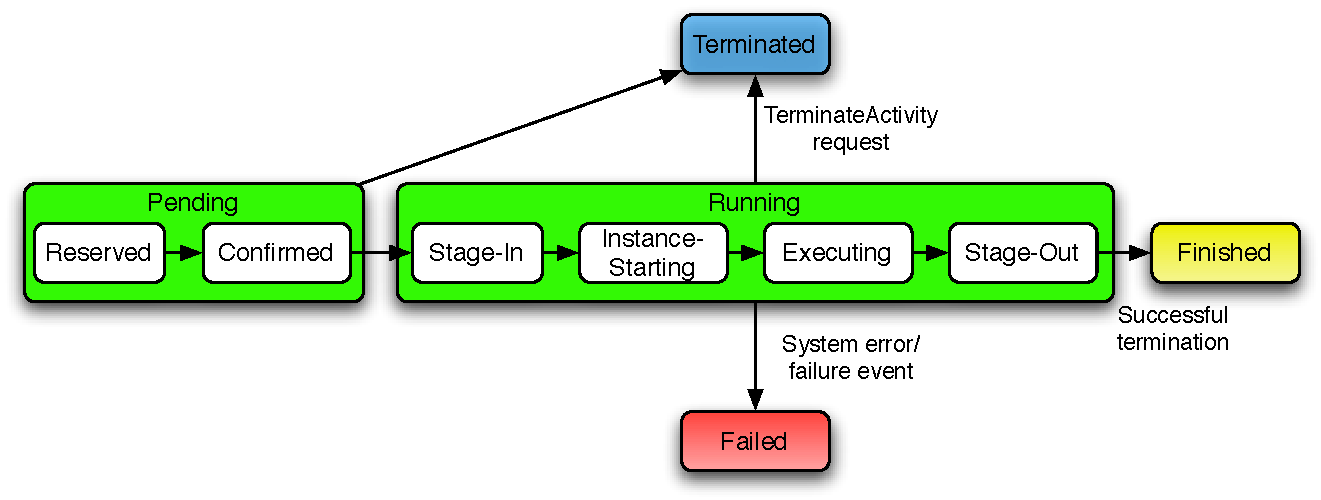
\includegraphics[scale=.55]{bes-job-model}
  \caption{The job-model used in the \gls{glo:XenBEE}}
  \label{fig:bes-job-model}
\end{figure}

The  implementation of  this model  builds up  on an  implementation  of a
\emph{Finite State  Machine} (\gls{glo:FSM}).  The  \texttt{Task} class, I
mentioned  earlier,  contains  a  reference  to an  instance  of  such  an
\gls{glo:FSM}. Each time  a state change is desired,  the \gls{glo:FSM} is
called with  an ``input'' signal. The \gls{glo:FSM}  then calls registered
functions that  implement the transition's  behavior. If, for  example, an
user wants to terminate his  activity, the \gls{glo:FSM} is presented with
a ``terminate-token''. The FSM  calls then specialized functions that deal
with the termination  request according to the current  state. That means,
distinct   functions    are   perhaps   called    when   traversing   from
\texttt{Pending:Reserved}    and    \texttt{Running:Executing}   to    the
\texttt{Terminated} state, respectively.

Some of the transitions  involve rather complex and time-consuming actions
(\eg file  transfers).   Those  complex  transitions are  represented  by
\emph{activity-objects}.    An   activity-object   is  an   object,   that
encapsulates  some behavior  along  with  a state  ---  commonly known  as
\emph{Function}-objects or \emph{Functors}.  I named them activity-objects
on  purpose, because they  are usually  executed by  a separate  thread of
control  in concurrency  to other  activities within  the  system. Another
reason for  encapsulating some of  the transitions in  activity-objects is
the possible intervention by an user.

The BES  model allows an  user to terminate  his activity at any  time. In
particular that means,  that any action belonging to  that activity, which
currently takes place  on the server, has to be  stopped or aborted.

Since the task-manager does not only create, but also manage the tasks, he
is responsible for stopping current activities of a task if he is asked to
do so.  For that reason, he is  in charge of a per task list that contains
all current activities  for that task. If the task-manage  is now going to
handle a request for termination of one of the tasks, he first cancels all
registered activity-objects before letting the task to change its state to
\texttt{Terminated}.

\begin{figure}[ht]
  \centering
  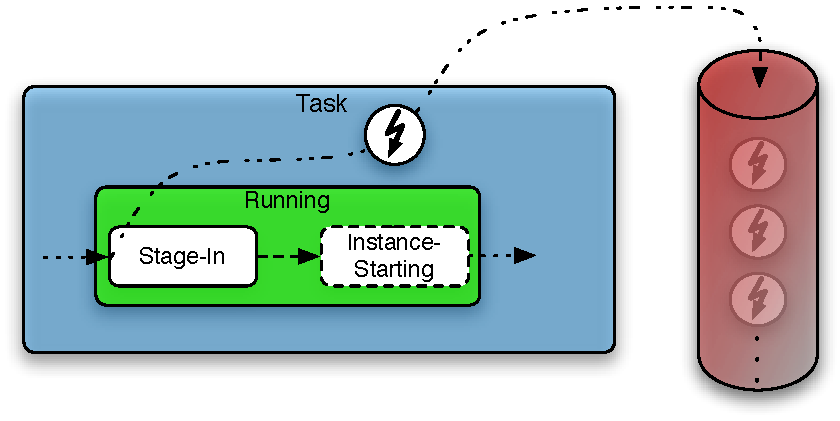
\includegraphics[scale=.55]{activity-queue}
  \caption{Handling of \emph{activity-objects} with an activity-queue.}
  \label{fig:activity-queue}
\end{figure}

The picture in Figure~\ref{fig:activity-queue} shows such an occasion. The
task (represented by  the blue box) is currently  in the \texttt{Stage-In}
sub-state  of \texttt{Running}  and is  awaiting the  availability  of its
required  files.  The  activity  which represents  here  the operation  of
staging files in is shown as  the encircled lightning bolt.  When the task
transitions  into  the \texttt{Stage-In}  state,  it  registers the  shown
activity with  the task-manager. The task-manager  in turn adds  it to his
queue of current activities (shown as the reddish tube in the right of the
picture).  When  the activity is  finished (figuratively speaking:  if the
activity exits through  the bottom of the tube), the  task may advance its
state to \texttt{Instance-Starting}, \ie it  can be attempted to start an
instance for this task.

Since  the  retrieval of  files  from  different  locations (specified  by
\gls{glo:URI}s  in the \gls{glo:JSDL})  may take  some time,  this example
also motivates  the usage of threads  to decouple other  activities of the
system  from these  steps. When  terminating  an activity,  the thread  is
signalled to abort whatever it is doing at the time.

\bigskip

Well,  the  whole cycle  through  which  a task  may  run  is depicted  in
Figure~\ref{fig:act-execute-task}  as  an   activity  diagram.   The  only
sub-activity that  cannot be aborted  at all is the  \emph{stop instance}
operation. That is because the  shutdown process of the underlying virtual
machine just cannot be cancelled or  reversed. That is also the reason to
not having an extra sub-state for that operation in the job-model.

The  process starts  with waiting  on  a ``ready-to-go''  signal, that  is
usually included  directly in the \texttt{Confirm} message  received by an
user,  but  can  also  be  given  in  a  subsequent  message  on  its  own
(\texttt{Start\-Activity})\footnote{the  communication  protocol  and  the
  messages           involved          are           discussed          in
  Section~\ref{sec:communication-protocol},
  \emph{\nameref{sec:communication-protocol}}.}.  The  next steps resemble
the previously discussed job-model. Of course, any of those activities may
\emph{fail}, which effectively  results in the failing of  the whole task.
The operations that are involved  when one of the sub-activities fails are
the  same  as  for  the  abortion of  that  sub-activity.   Actually,  the
\emph{stop  instance}  operation  cannot  fail  either,  since  it  always
possible to forcibly shut a virtual machine down.

\begin{figure}[ht]
  \centering
  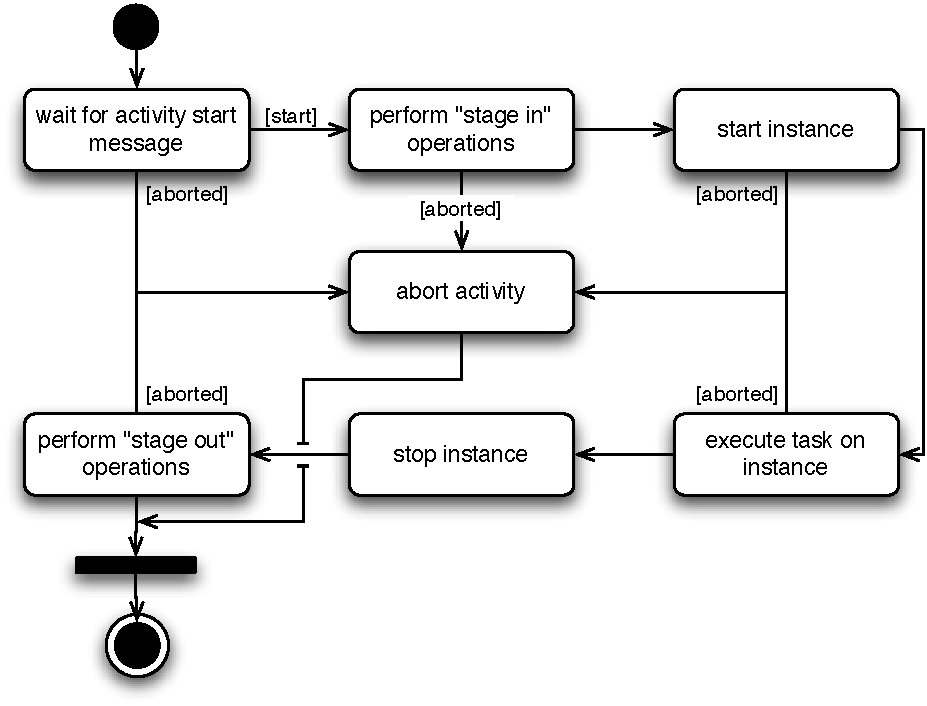
\includegraphics[scale=.55]{act-execute-task}
  \caption[Summary of executing a task]{Summary of the steps involved when executing a task.}
  \label{fig:act-execute-task}
\end{figure}

The \emph{start  instance} operation differs from the  other operations in
that two components are involved, the \emph{xbed} and the \emph{xbeinstd}.
The \emph{xbed}  first attempts  to start a  back-end instance (\eg  a Xen
virtual machine) and waits for the instance to be started, eventually.

After the instance  has been started, \ie the back-end  did not reject the
provided  configuration, the  \emph{xbed}, actually  the  thread executing
this  particular  activity,  waits  for  the \emph{xbeinstd}  to  send  an
\texttt{Instance\-Available}        message       back        to       the
\emph{xbed}. Figure~\ref{fig:act-start-instance} shows the details of that
particular activity.

\begin{figure}[ht]
  \centering
  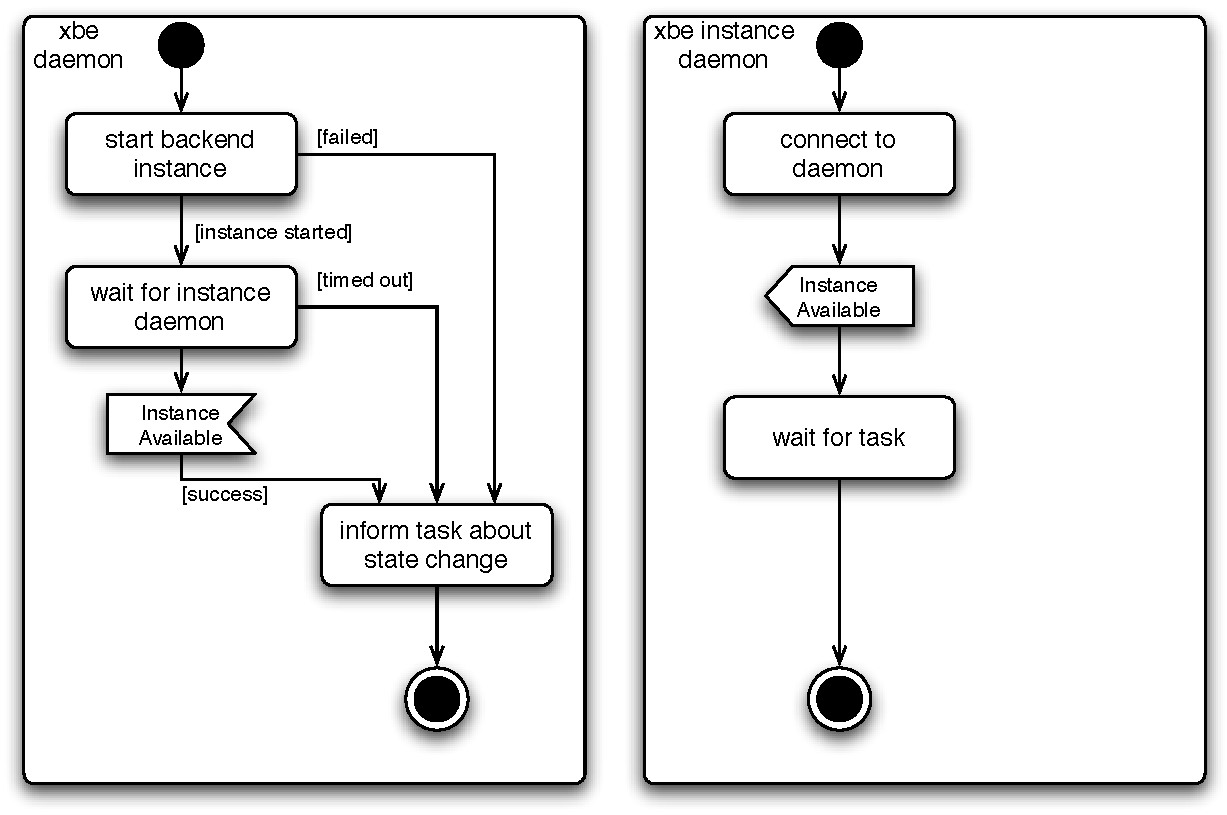
\includegraphics[scale=.55]{act-start-instance}
  \caption[Start Instance Activity]{The  \emph{xbed} waits for the virtual
    machine to  be available.   The availability of  a virtual  machine is
    made sure by waiting on a special message from the \emph{xbeinstd}.}
  \label{fig:act-start-instance}
\end{figure}


As you can see, there are  three different outcomes for this activity. The
instance can  be flagged as  available, which renders the  task eventually
executable,  the activity  can as  well be  aborted due  to a  request for
termination by  the user, or  the instance can  fail to start at  all. The
task's state will be changed according to the outcome of this activity.

After   sending   the   \texttt{Instance\-Alive}   notification   to   the
\emph{xbed},  the  \emph{xbeinstd}   waits  for  the  task's  description.
Additionally,  it will send  messages to  the \emph{xbed}  regularly, thus
making sure, that the virtual machine is still ``alive''.

\bigskip

The  next section deals  with the  staging operations  in more  detail. In
particular that means, how exactly  the files are retrieved, how files can
be compressed  to reduce  the required network-bandwidth  and how  one can
make sure that the file has been transfered correctly.

\subsection{Data Transfer Handling}
\label{sec:xbed:data-transfer}

The  handling  of data  transfer  covers the  staging  of  files into  the
execution environment and out from the execution environment, in this work
referred   to  as  ``stage-in''   and  ``stage-out''   respectively.   The
description  that  is  required  for  each of  the  staging  processes  is
completely  covered  within  the  \gls{glo:JSDL} document,  that  an  user
submitted  to the  execution  environment.  However,  some extensions  are
required,       those       will       be      handled       with       in
Section~\ref{sec:xen-based-submission}.

The  stage-in process  is  twofold.  The  first  part of  stage-in is  the
acquirement of files  that are mandatory for the  execution environment to
create    virtual    machine,    these    are    the    early    mentioned
\emph{\gls{glo:image}}  and  \emph{\gls{glo:kernel}}  files  (probably  an
\emph{\gls{glo:initrd}},  as well).   Without these  files, the  next part
cannot be started.

Well, the second part of the stage-in process handles the input files that
an  user had  specified for  his  application. These  definitions use  the
standard    \texttt{DataStaging}    element    of    the    \gls{glo:JSDL}
specification. These files are directly retrieved into the virtual machine
image, that  was previously obtained, hence  the two parts  of the staging
process.

All files, including the virtual machine specific ones, are referred to as
\emph{Uniform  Resource  Identifier}s  (\gls{glo:URI}s). That  means,  all
files must be ``somehow'' accessible by the \emph{xbed}.  An user can, for
instance,  specify files that  are located  on an  \texttt{HTTP} or  on an
\texttt{FTP} server ---  currently only these two protocols  and a special
URI to reference to cached  files are supported.  Those \gls{glo:URI}s are
then retrieved  by the  \emph{xbed} by using  the standard  mechanisms for
file retrieval based on  these protocols --- the library \texttt{libcurl},
which  relates to  the UNIX  \texttt{curl}  command is  used to  implement
download and upload.

\subsubsection{Support for compressed files}

As said before,  all input files related to  the application are retrieved
into  the virtual  machine image  directly. Consequently,  the  image must
provide enough  free space  to hold all  input and generated  output data,
which  can be  quite a  lot. Since  the  image is  an ordinary  file on  a
file-system, it can  easily consume unpredictable size. This  image has to
be  transfered  from  the user  (\ie  the  location  he specified  in  the
\gls{glo:JSDL}) to  the host on  which the \emph{xbed}  runs. Fortunately,
the image is nearly empty before transmitting it, since it contains only a
basic operating system installation  along with the user's application and
its dependencies.

The \emph{xbed} allows an user to submit compressed files. The compression
is extremely  useful when the file is  mostly ``empty'' as it  is the case
for the  image files, for  instance --- an  image file that was  $8$~GB in
size and contained  about $750$~MB data produced a  compressed file (using
\texttt{bzip2})  that was  about  $500$~MB  in size  only.   The usage  of
compressed files  reduces the  time needed to  transfer large,  but mostly
empty images significantly. The user is allowed to tag every file that she
submits to the execution environment  with the mode of compression and the
\emph{xbed} will decompress the file after retrieval.

\begin{figure}[ht]
  \centering
  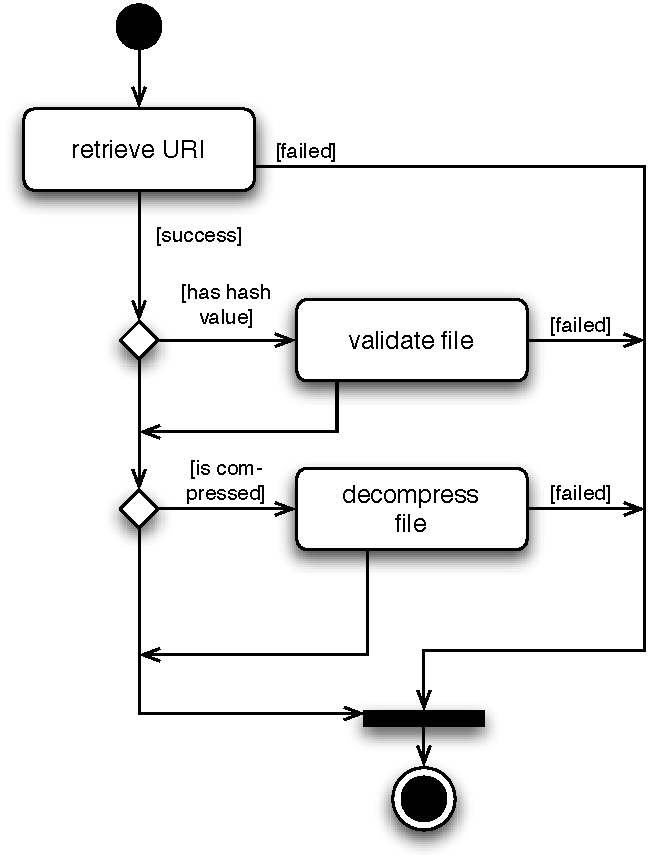
\includegraphics[scale=.55]{act-retrieve-file}
  \caption[File  Retrieval  Activity]{Steps  involved when  retrieving  an
    \gls{glo:URI}.}
  \label{fig:act-retrieve-file}
\end{figure}

\subsubsection{Support for validation of files}

Figure~\ref{fig:act-retrieve-file} shows the involved steps when a file is
retrieved by the \emph{xbed}. Another feature added to this process is the
validation of the retrieved data. If  an user wants to make sure, that the
file had not been modified in some way, she can provide a checksum and the
used    algorithm   along   with    the   \gls{glo:URI}.     Typically   a
\emph{cryptographic  hash   function}  is   used  to  compute   a  digital
fingerprint of the  data. All secure hash algorithms  that are provided by
the  Python  \texttt{hashlib} module  are  supported  (some examples  are:
\texttt{SHA1}, \texttt{SHA256}, \texttt{MD5}).

\subsubsection{The whole stage-in process}

The  stage-in   process  is   split  into  several   steps  as   shown  in
Figure~\ref{fig:act-stage-in}. The process always starts with the creation
of a \texttt{\gls{glo:chroot}} environment\footnote{The terms \emph{chroot
    environment}  and \emph{jail  environment} are  used interchangeably.}
within  the spool  directory that  has been  created for  that  task.  The
description of the  necessary files for a virtual  machine is contained in
an extra element within the task's \gls{glo:JSDL} description. An user can
either specify the required files (image, kernel and initrd) on its own or
he can specify a  \texttt{bzip2} compressed tar archive (``package'') that
contains these files.  Additionally, an user has the possibility to define
several executable scripts that  are uploaded to the execution environment
and get called at various stages of the stage-in process.

After  the package  or  the  virtual machine  files  have been  retrieved,
validated and  probably decompressed, the ``pre-setup''  hook is executed.
This  hook consists  of the  scripts that  were either  in the  package or
specified  by the user  and tagged  to be  in this  hook. All  scripts are
executed in the previously created \gls{glo:chrootenv} so that they cannot
access any file that does not belong to this task. Until now the execution
environment had  not touched the  image file, so  that one of  the scripts
could be used to decrypt the file, for instance.

\begin{figure}[ht]
  \centering
  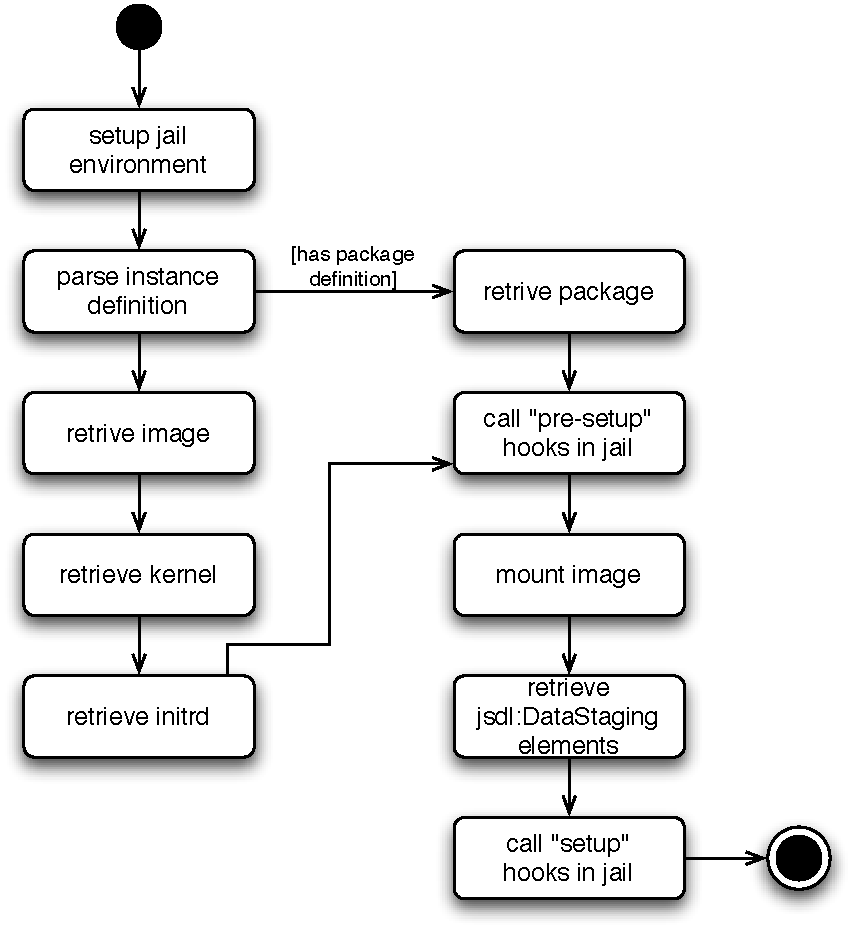
\includegraphics[scale=.55]{act-stage-in}
  \caption[Stage-In  Activity]{Overview  of  the  parts  of  the  stage-in
    activity.}
  \label{fig:act-stage-in}
\end{figure}

Now that all virtual machine specific files are available, the application
specific data can be retrieved. The \emph{xbed} assumes, that the image is
mountable by the UNIX \texttt{mount}  command and mounts it to a temporary
location within the jail environment.

All  JSDL-\texttt{DataStaging} elements that  define a  stage-in operation
are now handled with the  same retrieval mechanism as described above. The
paths that are used in the  job description are interpreted to be relative
to the mount point of the image.

Finally   the   ``setup''-hook  is   executed   using  the   user-supplied
scripts. These scripts  are given the path to  the image's mount-point and
can,  for  example,  decrypt  already  staged-in files  or  even  retrieve
additional input  data. If  everything went well,  the virtual  machine is
completely set up and can be started.

\subsubsection{Upload of files}

The upload of files from the execution environment to a location specified
by the user  is also accomplished by using  \gls{glo:URI}s. The process of
uploading a file is less  complicated than the retrieval process, since it
currently does  not involve compression or validation  directly.

The first step  after the virtual machine has been shut  down is again the
mounting of the image to a temporary location within the jail environment.
To provide  the possibility to  compress the files before  uploading them,
the ``cleanup'' hook is called before any of the actual staging operations
is called. The next step  is the handling of the JSDL-\texttt{DataStaging}
elements that  define a stage-out operation. The  only currently supported
protocols that can be  used for the upload are FTP and  HTTP. In the final
step of  the upload process the  ``post-cleanup'' hook is  called; to that
time,  all specified  staging  operations have  already been  successfully
performed and the image has been unmounted.

If everything  went well, all  stored data\footnote{this does  not include
  internal data structures (\eg exit-code).}  that belongs to this task is
destroyed (\ie  the spool directory will  be deleted) and the  task is put
into the \texttt{Finished} state.

\subsection{Caching Of Arbitrary Files}
\label{sec:caching}

Compression   of  files   can   decrease  the   deployment  time   already
significantly, but  to avoid  long-distance transfers over  an unspecified
network connection, the  caching of files on the  server side is required,
this    follows    strictly    from    the    \emph{locality    principle}
\cite{locality-principle}.  The \emph{xbed} supports this by providing the
user with a  simple data-cache incorporated into the  system.  The user is
able to store  arbitrary data on the server prior submitting  a job to the
system. This makes the initialization  of a virtual machine for often used
images a lot faster compared  to always retrieving them over a potentially
slow network connection.

\subsubsection{Adding data to the cache}

An  user  adds  files  to  the  execution  environment  by  specifying  an
\gls{glo:URI} that can be retrieved by the \emph{xbed}.  This will usually
be the same \gls{glo:URI} the user would have given in his job description
(\eg a location  on some FTP or HTTP server).  The \emph{xbed} attempts to
retrieve the given \gls{glo:URI} and adds a new entry to a database.

Actually the  complete mechanism  of caching is  implemented in  a special
component  within  the  \emph{xbed}  on   its  own.   The  cache  uses  an
\gls{glo:SQL}-database  to store information  about the  cached data  in a
persistent way. An user can add two different pieces of information to the
data he wants to have cached.  The first is the \textbf{type} of the data,
which can  be one  of \texttt{image}, \texttt{kernel},  \texttt{initrd} or
\texttt{data},  where the  \texttt{data} type  is just  a  placeholder for
arbitrary data  that does not fit  into one of the  other categories.  The
second piece of information is a \textbf{description}, that can be used to
describe the data in more detail,  \eg the version of a specific kernel, a
list of the applications that are installed within an image or the type of
compression   if  the   data   had  been   compressed.   Additionally   an
\texttt{SHA1}  digital fingerprint  of the  data is  computed  and stored,
along with the provided information, in the database.

The  cache-component assigns  each  entry an  unique  identifier based  on
\gls{glo:UUID}s, this identifier can later  be used in an \gls{glo:URI} to
refer to that  entry.  When using the \emph{xbe} command  line tool to add
data to  the cache, the \gls{glo:URI}  of the newly created  entry will be
printed on the screen upon success.

\subsubsection{Discovering cache entries}

Well, the first way of ``discovering''  an entry of the cache is simply to
write  down  the \gls{glo:URI}  one  has  received  upon addition  of  the
entry. But  that is not always  feasible, since the entry  could be shared
among several users  who do not know each other  --- say, an administrator
or provider of a  virtual machine image added it to the  cache, so that it
can be used by several, to that time unknown, users.

The  discovery of  cached entries  is  implemented in  the \emph{xbed}  by
simply providing the  user with a list of all  entries. This list contains
most importantly the \gls{glo:URI} of the  entry, the type of data and the
description the submitter had given.

\begin{figure}[ht]
  \centering
  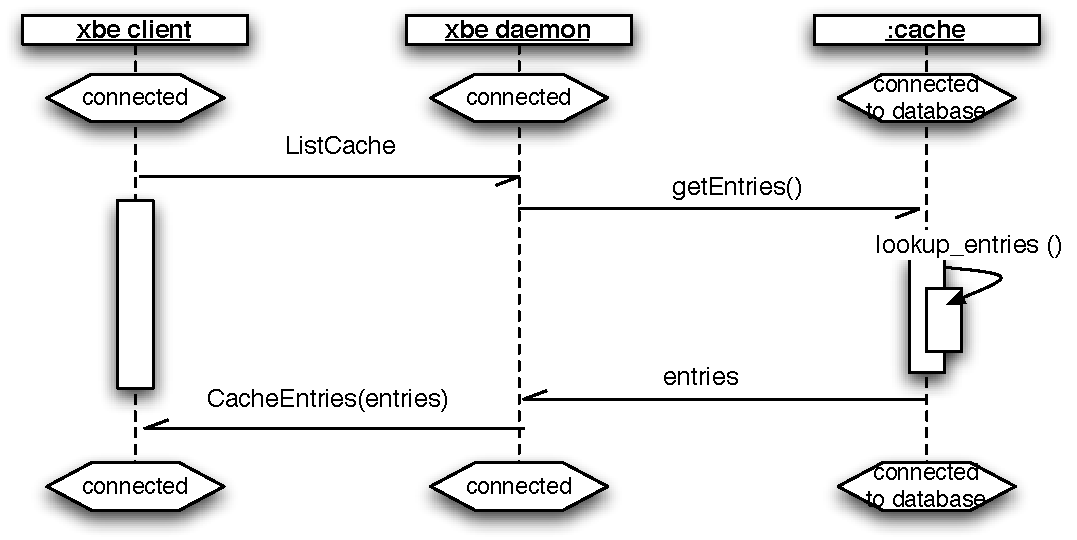
\includegraphics[scale=.55]{msc-list-cache}
  \caption[MSC List Cache Entries]{TODO: fill me in}
  \label{fig:msc-list-cache}
\end{figure}

The      \emph{Message     Sequence     Chart}      (\gls{glo:MSC})     in
Figure~\ref{fig:msc-list-cache} shows  the messages that  are sent between
the  client and  the server.   The client  requests a  list of  all cached
entries  by sending  the \texttt{ListCache}  message. Thereupon  makes the
\emph{xbed} a call to the cache-component  that provides him a list of all
entries. This list is eventually  transformed into an XML-message and sent
back to the client.  A sample output of the \texttt{xbe showcache} command
is shown in the following listing:

\bigskip

\begin{center}
  \begin{minipage}{.75\textwidth}
    \begin{lstlisting}[captionpos=b,backgroundcolor=\color{listingcolor},frame=lines,numbers=left,numberstyle=\tiny,caption={\emph{xbe} output of cache entries.},label={lst:xbe-listcache-out}]
<CacheEntries with 1 entry:
{'cache://xbe-file-cache/adfd0a99-4761-4816-8902-db8d62c8e482':
  {'description': 'Ubuntu kernel (2.6)',
   'hash': '732ca16f330c2c382e83cb997f5e027687a285aa',
   'type': 'kernel'}}
>
    \end{lstlisting}
  \end{minipage}
\end{center}

\subsubsection{Using cache entries}

Cache  entries can  be used  rather  easy. The  user is  just required  to
specify  the  \gls{glo:URI} of  a  cache  entry  instead of  the  original
\gls{glo:URI}.   The \emph{xbed} will  lookup the  specified \gls{glo:URI}
during the  stage-in process and  retrieve the data  from the cache,  if a
valid entry  could be found. The  same retrieval mechanism  applies to the
cached entries, so that compression  and validation can be used with them,
too.


\subsection[Xen-based Submission Description Language]{Xen-based Submission Description Language (XSDL)}
\label{sec:xen-based-submission}

an extension to the \gls{glo:JSDL}


\section[Xen-based Execution Instance Daemon]{Xen-based Execution Instance Daemon (xbeinstd)}
\label{sec:xbeinstd}

\begin{itemize}
\item notifies xbed when instance is up (\ie network connectivity)
\item keep-alive
\item input files are already available
\item parses jsdl
\item sets working directory
\item redirects standard input/output/error to the files in jsdl (or /dev/null)
\item starts task when the xbed notifies
\item passes arguments specified in jsdl
\item notifies xbed when application has finished (shutdown may be initialized)
\end{itemize}
foo bar

\section{The Communication Protocol}
\label{sec:communication-protocol}

\begin{itemize}
\item make reservation
\item confirm reservation (jsdl) +/- start
\item submit whole job (make res + confirm)
\item terminate activity
\item status request
\item add cache entry
\item security establishment (certificates, encryption, signing)
\item stomp
\end{itemize}

\subsection{STOMP}
\label{sec:protocol:stomp}

\subsection{MSCs}

\begin{figure}[ht]
  \centering
  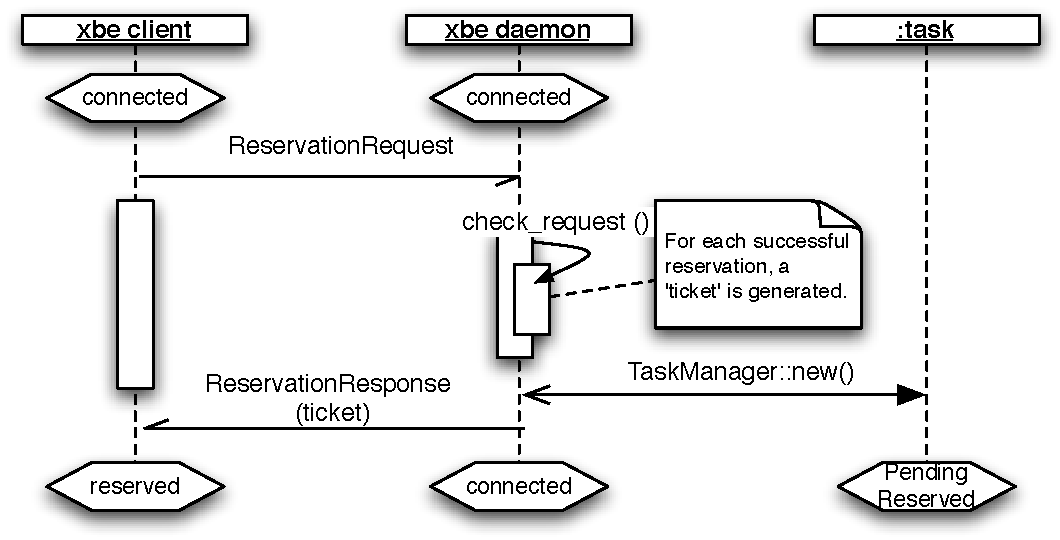
\includegraphics[scale=.75]{msc-reserve}
  \caption[MSC Make Reservation]{TODO: fill me in}
  \label{fig:msc-reserve}
\end{figure}

\begin{figure}[ht]
  \centering
  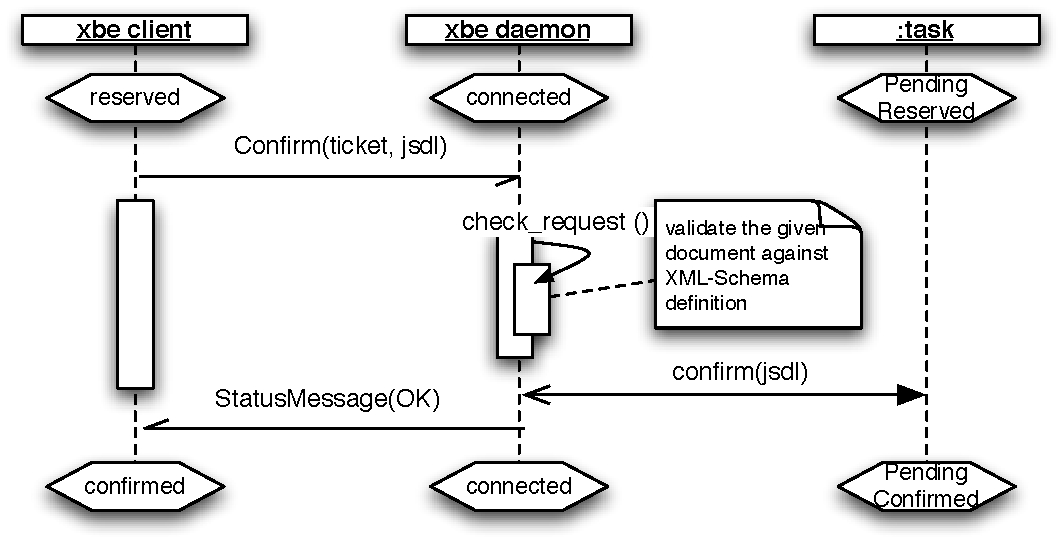
\includegraphics[scale=.75]{msc-confirm}
  \caption[MSC Confirm Reservation]{TODO: fill me in}
  \label{fig:msc-confirm}
\end{figure}

\begin{figure}[ht]
  \centering
  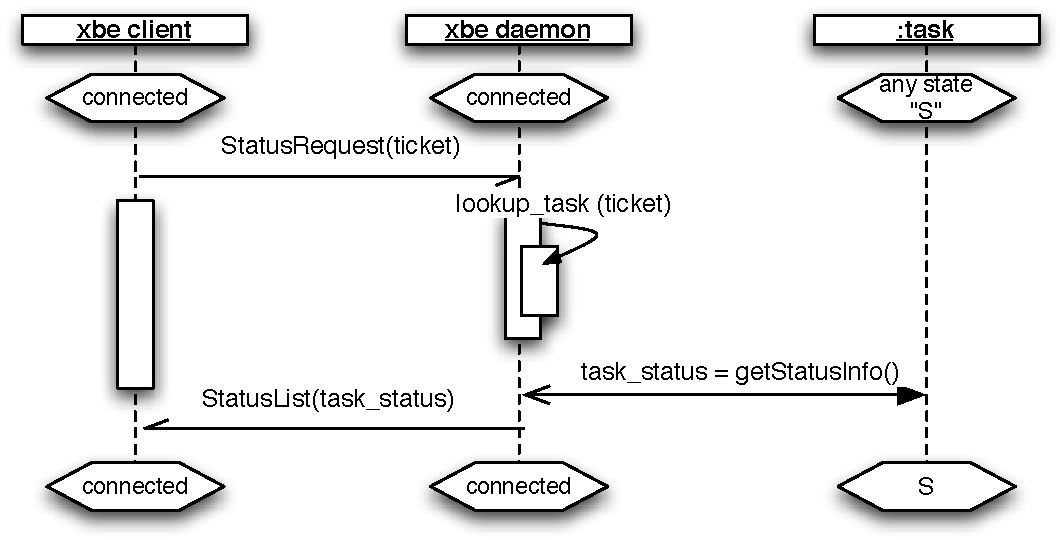
\includegraphics[scale=.75]{msc-status-request}
  \caption[MSC Request Task Status]{TODO: fill me in}
  \label{fig:msc-status-request}
\end{figure}

\begin{figure}[ht]
  \centering
  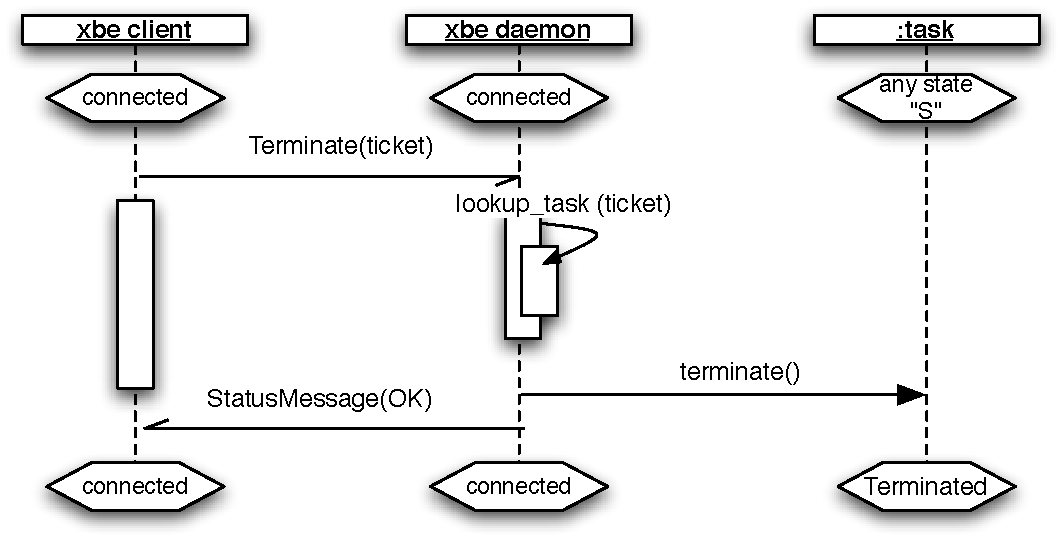
\includegraphics[scale=.75]{msc-terminate}
  \caption[MSC Terminate Task Request]{TODO: fill me in}
  \label{fig:msc-terminate}
\end{figure}

\subsection{Network Topology}
\label{sec:network-topology}

\begin{itemize}
\item simple topology: just one mqs (preferably on the xbed-host)
\item advanced topology: many mqs with configured forwarding
\item avoids common problems that arise with NAT and firewall policies
\item xbeinstd and possibly the application use the same mqs as the xbed
\end{itemize}

\begin{figure}[ht]
  \centering
  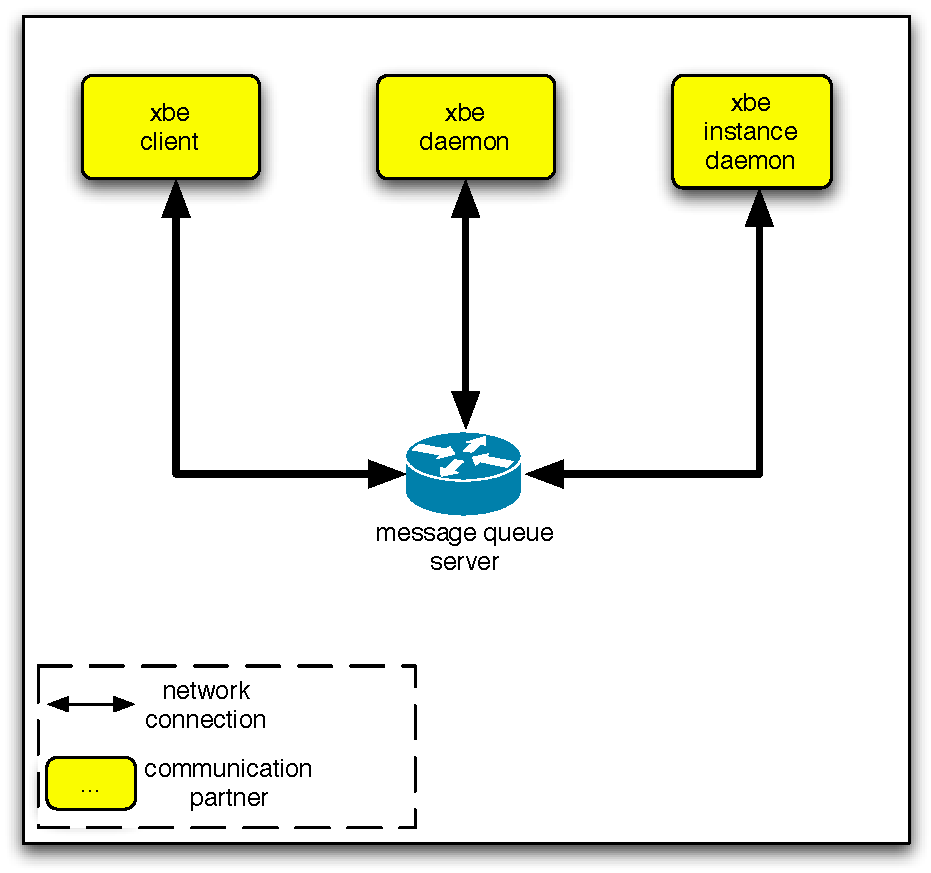
\includegraphics[scale=.75]{simple-network-topology}
  \caption[Network  Topology   (simple)]{The  simplest  network  topology,
    consisting of  only one Message  Queue Server and  three communication
    partners.}
  \label{fig:simple-net-top}
\end{figure}

\begin{figure}[ht]
  \centering
  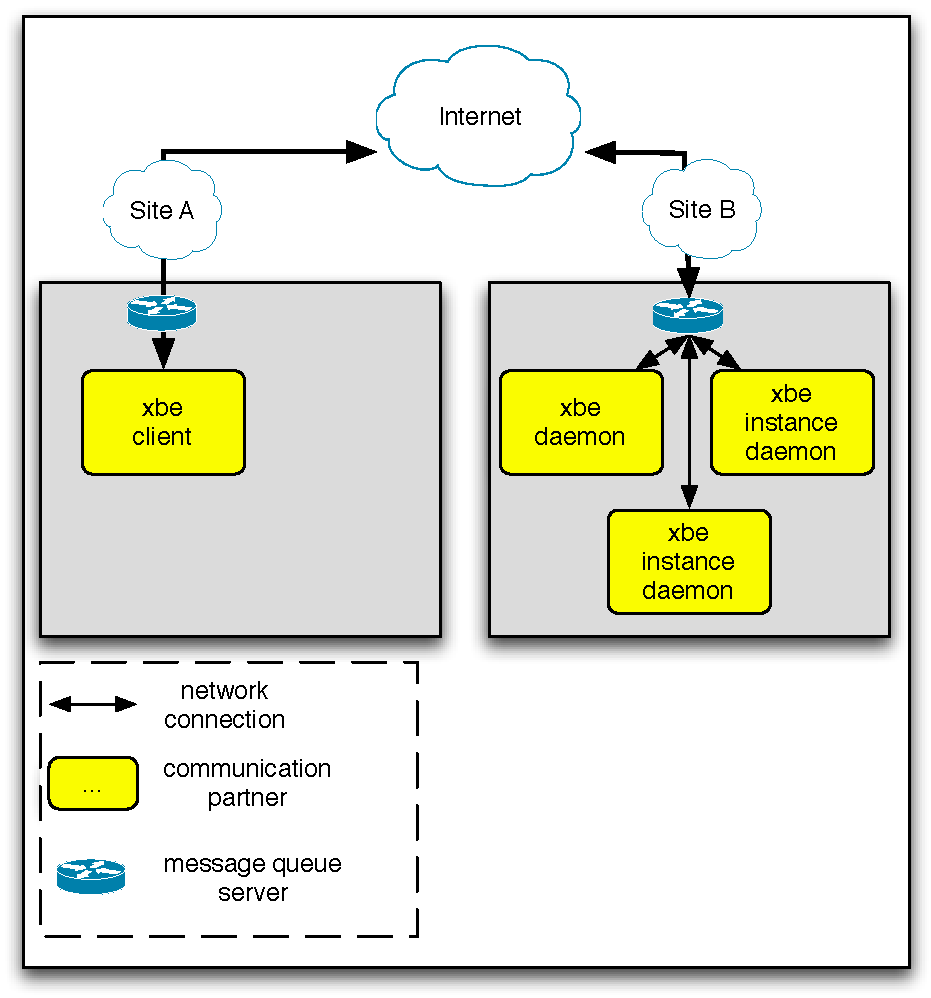
\includegraphics[scale=.75]{network-topology}
  \caption[Network  Topology]{TODO: fill me in}
  \label{fig:net-top}
\end{figure}

\subsection{Security}
\label{sec:security}

\begin{itemize}
\item symmetric encryption one-time key
\item signing of whole message
\item encryption of body
\item xml-message-security
\end{itemize}

\begin{figure}[ht]
  \centering
  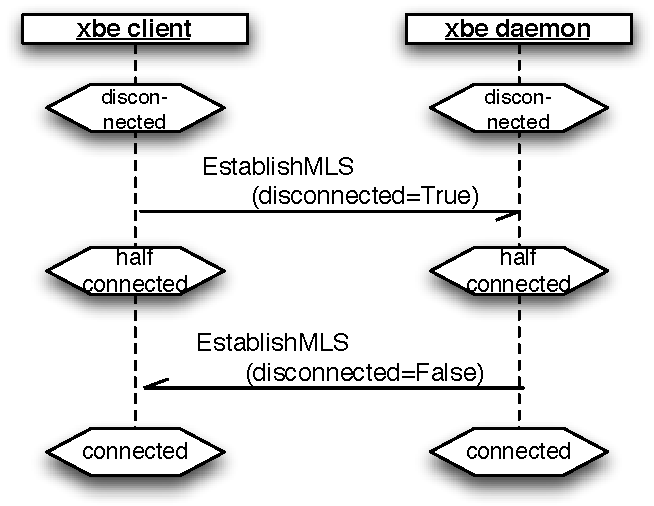
\includegraphics[scale=.75]{msc-establish-mls}
  \caption[MSC Message Layer Security]{TODO: fill me in}
  \label{fig:msc-establish-mls}
\end{figure}


\begin{figure}[ht]
  \centering
  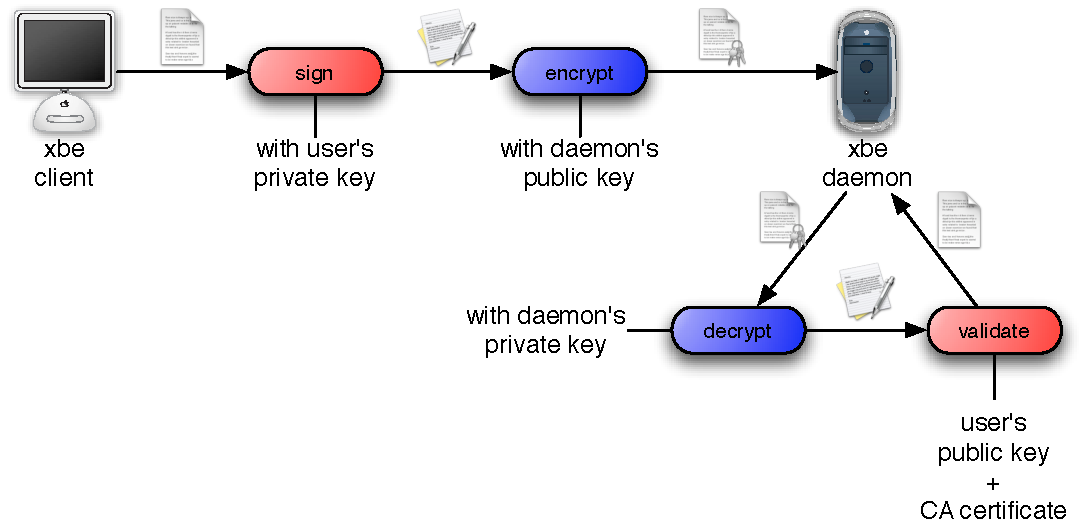
\includegraphics[scale=.75]{message-layer-security}
  \caption[Message Layer Security]{TODO: fill me in}
  \label{fig:net-mls}
\end{figure}

\subsubsection{m2crypto / openssl}

\begin{itemize}
\item problems with m2crypto on 64bit architecture
\item both are currently incompatible to each other
\item both sides (client/server) have to use the same --- either m2 or
  direct openssl
\end{itemize}

%%% Local Variables: 
%%% mode: latex
%%% TeX-master: "main"
%%% End: 
